%%%%%%%%%%%%%%%%%%%%%%%%%%%%%%%%%%%%%%%%%%%%%%%%%%%%%%%%%%%%%%%%%%%%%%%%%%%
%% This file is part of the book
%%
%% Algorithmic Graph Theory
%% http://code.google.com/p/graph-theory-algorithms-book/
%%
%% Copyright (C) 2009, 2010, 2011 Minh Van Nguyen <nguyenminh2@gmail.com>
%%
%% See the file COPYING for copying conditions.
%%%%%%%%%%%%%%%%%%%%%%%%%%%%%%%%%%%%%%%%%%%%%%%%%%%%%%%%%%%%%%%%%%%%%%%%%%%

\documentclass{article}

\usepackage{amsmath}
\usepackage{pgfplots}
\usetikzlibrary{external}
\tikzexternalize{Milgram-small-world-experiment-results}

\begin{document}

\begin{figure}
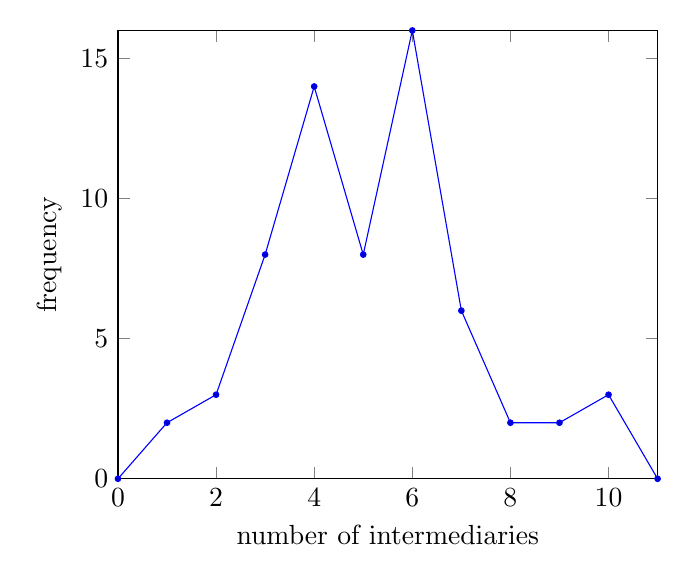
\begin{tikzpicture}
[every mark/.append style={scale=0.5}]
\begin{axis}[%
  enlargelimits=false,%
  xlabel=\text{number of intermediaries},%
  ylabel=\text{frequency}%
]
\addplot+[sharp plot] coordinates
{(0,0)  (1,2)  (2,3) (3,8) (4,14)%
 (5,8)  (6,16) (7,6) (8,2) (9,2)%
 (10,3) (11,0)
};
\end{axis}
\end{tikzpicture}
\end{figure}

\end{document}
